\cleardoublepage
\chapter{Testing and Verification}
\label{ch:testing}

The following section covers the testing and verification techniques performed on the compiler. This was carried out to ensure that the generated Java code can be compiled and executed in a way that satisfies the design aims and programming needs.

\section{Generated Java Code Analysis}

One of the methods used to perform code verification was the analysis of the generated Java code. In particular, for the global protocol classes, it is important to ensure that all participant fields are generated within the class, so that operations can be called on these participants. These fields need to be initialised with the correct values. Further, it is also crucial that the compiler successfully assigns modifier flags to these participants, as well as to the protocol class itself. These flags are defined by the user for the protocol class and implicitly set by the compiler to \LST{public} for the participant members. Finally, the appropriate interfaces and superclasses need to be integrated into the class definitions, so that the necessary methods are inherited in order to be used by the programmers.

In a normal setting, all these can be verified by checking the generated Java source code output, for all these annotations. This involves checking, whether the fields have initialising code in their definitions, whether the keywords \LST{public, private, extends} and \LST{implements} are present, as well as whether the general structure of the code is equal to the desired one.

We did however, encounter a case where all these checkpoints were achieved, but access to the member fields within the implementation code was denied by the compiler with a \LST{ClassNotFound} exception. We used the technique described in the following \autoref{sec:debugmode} to specify the problem and find an appropriate solution.

\section{Integrated IDE Debug Mode}
\label{sec:debugmode}

The development of MPSJ was facilitated by the use of Eclipse IDE as the main programming tool. Eclipse has an inbuilt debug mode, which allows the programmer to analyse the data flows between the methods and check intermediary values of the variables as they are being processed.

The problem mentioned above was followed through and it turned out the generated global participant fields were created with an \LST{\{amb\}} annotation, showing that the nodes are ambiguous to the compiler. The class fields were added during the \LST{SJProtocolTranslator} compiler pass, which was scheduled after the disambiguation pass. To rectify the error we moved the addition of the global participants into the global protocol class constructor and left the initialisation of these fields factored out in the \LST{SJProtocolTranslator} pass.

However, the problems encountered with this situation encouraged us to develop a debugging framework which ensures that the generated global protocol class adheres to our requirements. The sequence of verifications is depicted in \autoref{fig:debugging}.

\begin{figure}[H]
\begin{center}
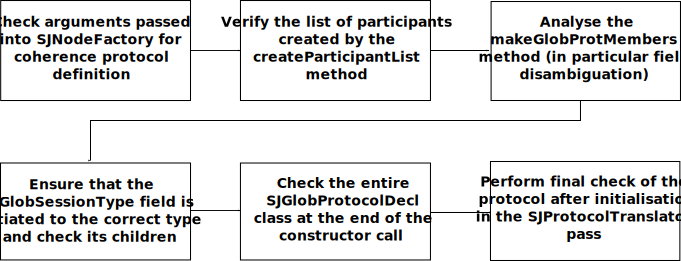
\includegraphics[width=0.8\textwidth]{debugging}
\caption{Global protocol declaration debugging framework}
\label{fig:debugging}
\end{center}
\end{figure}

We begin the verification by checking that the arguments passed into the node factory correspond to the initial global session type definition interpreted by the parser. We then analyse the procedures in the \LST{createParticipantList} which is the participant inference method in order to verify that the created list contains all members without any repetitions. Based on this list, the method \LST{makeGlobProtocolMembers} creates the fields of the class. At this stage it needs to be ensured that all members are disambiguated to avoid the problems mentioned before. Following that, we check whether the \LST{SJGlobSessionType} member of the protocol class is initiated properly and whether all its children are attached to it. Finally, we perform two final verifications, one on the exit from the global protocol constructor and one after the \LST{SJProtocolTranslator} pass, in which the participant fields are initialised. If at any stage our analysis showed any problems, we aborted the progress and investigated the issues we found.

We decided to develop such a rigorous framework for the protocol declaration because of its importance for our implementation and all programmers using it. As it is the central point of interaction, it needs to be verified via a structured approach that all its functionality is safely achieved after the compiler has finished processing the data.
